\documentclass[a4paper,12pt]{article}
\usepackage[a4paper,top=1.3cm,bottom=2cm,left=1.5cm,right=1.5cm,marginparwidth=0.75cm]{geometry}
\usepackage{cmap}
\usepackage{mathtext}
\usepackage[T2A]{fontenc}
\usepackage[utf8]{inputenc}
\usepackage[english,russian]{babel}
\usepackage{siunitx}
\usepackage{enumitem}
\usepackage{placeins}

\usepackage{graphicx}
\usepackage{subcaption}
\usepackage{amsmath}

\usepackage{wrapfig}
\usepackage{tabularx}
\usepackage{multirow}

\usepackage{hyperref}
\usepackage[rgb]{xcolor}
\hypersetup{colorlinks=true,urlcolor=blue}
\usepackage{amsmath,amsfonts,amssymb,amsthm,mathtools}
\usepackage{mathtools}
\usepackage{icomma}
\mathtoolsset{showonlyrefs=false}
\usepackage{euscript}
\usepackage{mathrsfs}
\DeclareMathOperator{\sgn}{\mathop{sgn}}
\newcommand*{\hm}[1]{#1\nobreak\discretionary{}
{\hbox{$\mathsurround=0pt #1$}}{}}

\newcommand\labname{Генераторы синусоидальных колебаний с кварцевой стабилизацией частоты}
\newcommand\labnumber{5}

\author{Макаров Лев Евгеньевич}
\title{Лабораторная работа №\labnumber\\\labname}
\date{\today}

\makeatletter
\AddEnumerateCounter{\asbuk}{\russian@asbuk@alph}{щ}
\makeatother

\begin{document}

\begin{titlepage}
    \begin{center}
        {\large МОСКОВСКИЙ ФИЗИКО-ТЕХНИЧЕСКИЙ ИНСТИТУТ (НАЦИОНАЛЬНЫЙ ИССЛЕДОВАТЕЛЬСКИЙ УНИВЕРСИТЕТ)}
    \end{center}
    \begin{center}
        {\large Физтех-школа фотоники, электроники и молекулярной физики}
    \end{center}

    \vspace{4.5cm}
    {\huge
        \begin{center}
            {\bf Отчёт о выполнении лабораторной работы \labnumber}\\
            \labname
        \end{center}
    }
    \vspace{2cm}
    \begin{flushright}
        {\LARGE Автор:\\ Макаров Лев Евгеньевич\\
        \vspace{0.2cm}
        Б04-306}
    \end{flushright}
    \vspace{8cm}
    \begin{center}
        Долгопрудный 2026
    \end{center}
\end{titlepage}

\section{Введение}

\textbf{Цель работы:} ознакомиться со схемами генераторов синусоидальных колебаний, построенных на основе усилителей с обратной связью, в том числе генераторов с кварцевой стабилизацией частоты.

В работе исследуется резонансный усилитель и два кварцевых генератора. В первом генераторе кварцевый резонатор используется на частоте последовательного резонанса, во втором -- как эквивалентная индуктивность в трехточечной схеме.

\section{Выполнение работы}

\subsection*{Резонансный усилитель}

\begin{enumerate}
    \item Соберем схему резонансного усилителя согласно рис. \ref{pic:ustan-6-1}. Выходом усилителя является напряжение $U_\text{out}$, а напряжение $U_\text{in}$ используется как сигнал цепи обратной связи.
\end{enumerate}

\begin{figure}[h]
    \centering
    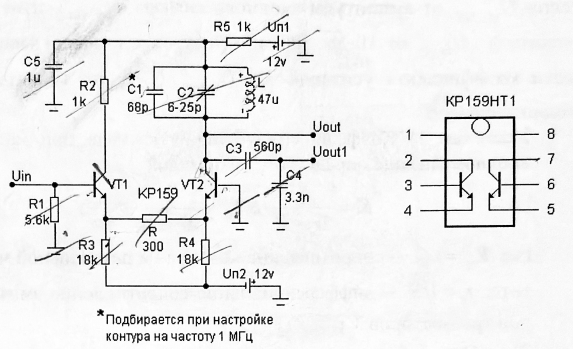
\includegraphics[width=0.75\textwidth]{pictures/ustan-6-1.png}
    \caption{Схема резонансного усилителя}
    \label{pic:ustan-6-1}
\end{figure}

Использованные элементы схемы представлены в таблице \ref{tab:params-6-1}.

\begin{table}[!h]
    \centering
    \caption{Параметры элементов резонансного усилителя}
    \label{tab:params-6-1}
    \begin{tabular}{|l|l|l|l|l|l|}
        \hline
        $R_1$, кОм & $R_2$, кОм & $R_3$, кОм & $R_4$, кОм & $R_5$, кОм & $R$, Ом \\ \hline
        5.492 & 0.986 & 18.09 & 17.973 & 0.9825 & 294.7 \\ \hline
        $C_1$, пФ & $C_2$, пФ & $C_3$, пФ & $C_4$, нФ & $C_5$, мкФ & $L$, мкГн \\ \hline
        68 & 20 & 561 & 3.32 & 6.05 & 47 \\ \hline
    \end{tabular}
\end{table}

\begin{enumerate}[resume]
    \item Измерим потенциалы на электродах транзисторов при $U_{\text{П}2} = -10~\text{В}$. Результаты занесем в таблицу \ref{tab:transistors-6-1}.
\end{enumerate}

\begin{table}[!h]
    \centering
    \caption{Потенциалы на электродах транзисторов}
    \label{tab:transistors-6-1}
    \begin{tabular}{|l|l|l|l|}
        \hline
        Транзистор & $U_\text{К}$, В & $U_\text{Э}$, В & $U_\text{Б}$, В \\ \hline
        VT1 & 9.9941 & -0.6014 & -0.0020 \\ \hline
        VT2 & 9.9941 & -0.5990 & -0.0005 \\ \hline
    \end{tabular}
\end{table}

По измеренным потенциалам найдем токи эмиттеров:

\begin{equation*}
    I_{\text{Э}1} = \cfrac{U_{\text{Э}1} - U_{\text{П}2}}{R_3} = 0.520~\text{мА},
    \qquad
    I_{\text{Э}2} = \cfrac{U_{\text{Э}2} - U_{\text{П}2}}{R_4} = 0.523~\text{мА}.
\end{equation*}

Средний ток коллектора

\begin{equation*}
    I_\text{К} \approx \cfrac{I_{\text{Э}1} + I_{\text{Э}2}}{2} = 0.521~\text{мА}.
\end{equation*}

При $U_T = 25~\text{мВ}$ крутизна транзисторов равна

\begin{equation*}
    S = \cfrac{I_\text{К}}{U_T} = 0.021~\Omega^{-1}.
\end{equation*}

\begin{enumerate}[resume]
    \item Подадим входной синусоидальный сигнал и найдем резонансную частоту по максимуму выходного напряжения. По измерениям $f_\text{р} = 1.01~\text{МГц}$.

    \item На резонансной частоте снимем амплитудную характеристику усилителя. Результаты представлены в таблице \ref{tab:data-6-1-3}.
\end{enumerate}

\begin{table}[!h]
    \centering
    \caption{Амплитудная характеристика резонансного усилителя}
    \label{tab:data-6-1-3}
    \begin{tabular}{l|l|l||l|l|l}
        \hline
        $U_\text{in}$, мВ & $U_\text{out}$, мВ & $K$ & $U_\text{in}$, мВ & $U_\text{out}$, мВ & $K$ \\ \hline
        10 & 80 & 8.00 & 260 & 1985 & 7.63 \\
        20 & 160 & 8.00 & 270 & 2030 & 7.52 \\
        30 & 239 & 7.97 & 280 & 2097 & 7.49 \\
        40 & 319 & 7.98 & 290 & 2165 & 7.47 \\
        50 & 410 & 8.20 & 300 & 2235 & 7.45 \\
        60 & 490 & 8.17 & 310 & 2300 & 7.42 \\
        70 & 572 & 8.17 & 320 & 2363 & 7.38 \\
        80 & 655 & 8.19 & 330 & 2420 & 7.33 \\
        90 & 725 & 8.06 & 340 & 2480 & 7.29 \\
        100 & 807 & 8.07 & 350 & 2537 & 7.25 \\
        110 & 885 & 8.05 & 360 & 2597 & 7.21 \\
        120 & 970 & 8.08 & 370 & 2659 & 7.19 \\
        130 & 1055 & 8.12 & 380 & 2712 & 7.14 \\
        140 & 1135 & 8.11 & 390 & 2769 & 7.10 \\
        150 & 1212 & 8.08 & 400 & 2831 & 7.08 \\
        160 & 1292 & 8.08 & 410 & 2892 & 7.05 \\
        170 & 1370 & 8.06 & 420 & 2970 & 7.07 \\
        180 & 1449 & 8.05 & 430 & 3053 & 7.10 \\
        190 & 1527 & 8.04 & 440 & 3130 & 7.11 \\
        200 & 1600 & 8.00 & 450 & 3195 & 7.10 \\
        210 & 1665 & 7.93 & 460 & 3237 & 7.04 \\
        220 & 1722 & 7.83 & 470 & 3296 & 7.01 \\
        230 & 1785 & 7.76 & 480 & 3320 & 6.92 \\
        240 & 1852 & 7.72 & 490 & 3350 & 6.84 \\
        250 & 1915 & 7.66 & 500 & 3395 & 6.79 \\ \hline
    \end{tabular}
\end{table}

\begin{figure}[!h]
    \centering
    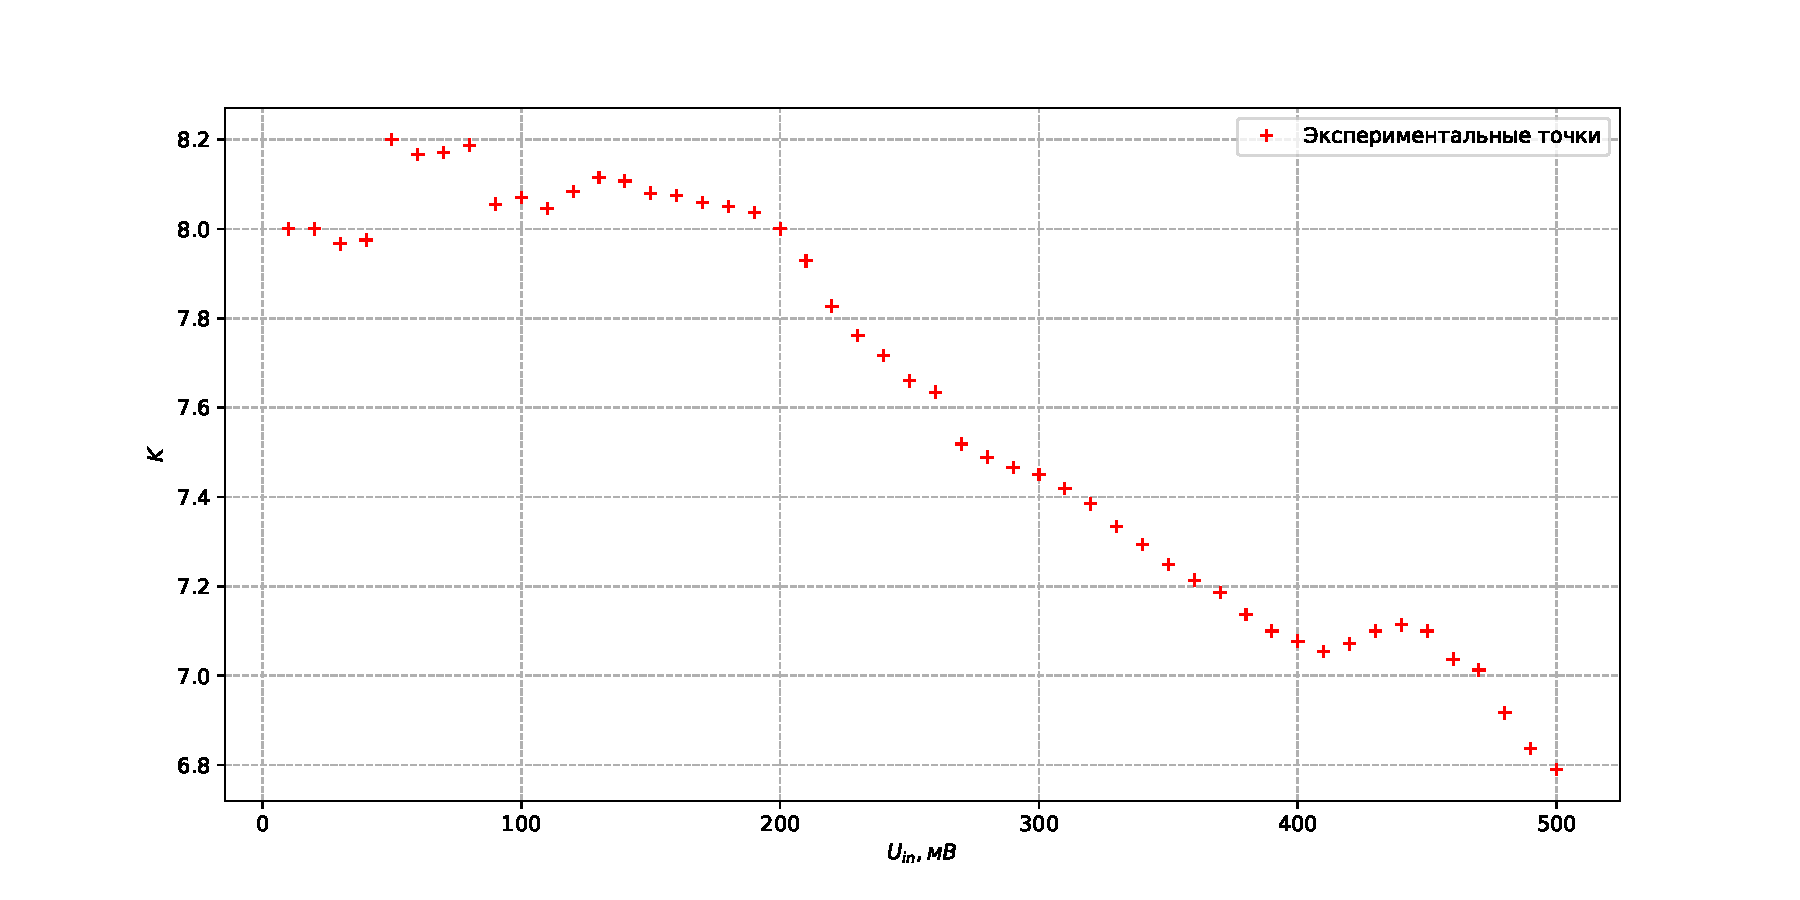
\includegraphics[width=\textwidth]{pictures/6_1_3_graph.pdf}
    \caption{Зависимость коэффициента усиления $K$ от амплитуды входного сигнала}
    \label{pic:graph-6-1-3}
\end{figure}

Из графика видно, что при малых входных амплитудах коэффициент усиления близок к постоянному значению $K \approx 8$. При дальнейшем увеличении амплитуды входного сигнала начинается насыщение, и коэффициент усиления уменьшается.

\begin{enumerate}[resume]
    \item Замкнем эмиттеры транзисторов, что соответствует случаю $R = 0$, и повторим измерение резонансного коэффициента усиления. Данные представлены в таблице \ref{tab:data-6-1-4}.
\end{enumerate}

\begin{table}[!h]
    \centering
    \caption{Амплитудная характеристика при $R = 0$}
    \label{tab:data-6-1-4}
    \begin{tabular}{|l|l|l|}
        \hline
        $U_\text{in}$, мВ & $U_\text{out}$, мВ & $K$ \\ \hline
        500 & 6738 & 13.48 \\ \hline
        430 & 6738 & 15.67 \\ \hline
        350 & 6574 & 18.78 \\ \hline
        270 & 6265 & 23.20 \\ \hline
        200 & 5750 & 28.75 \\ \hline
        130 & 4697 & 36.13 \\ \hline
        50 & 2038 & 40.76 \\ \hline
    \end{tabular}
\end{table}

\begin{figure}[!h]
    \centering
    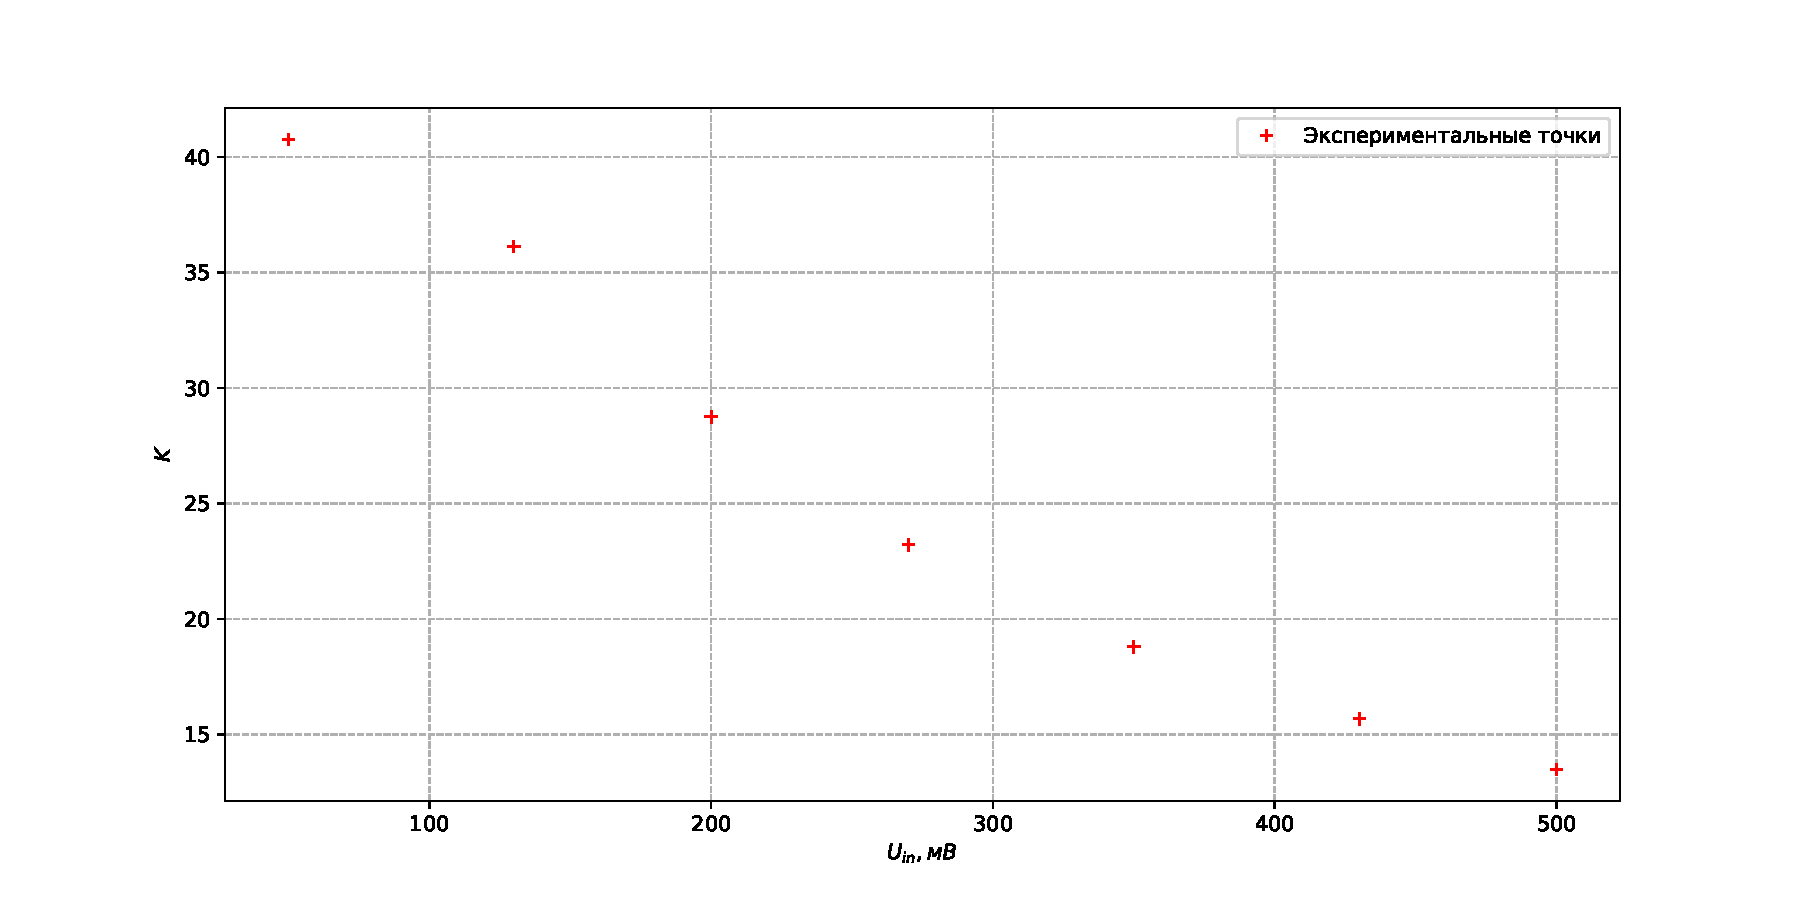
\includegraphics[width=\textwidth]{pictures/6_1_4_graph.pdf}
    \caption{Зависимость коэффициента усиления $K$ от амплитуды входного сигнала при $R = 0$}
    \label{pic:graph-6-1-4}
\end{figure}

При коротком замыкании эмиттеров отрицательная обратная связь по эмиттерной цепи уменьшается, поэтому резонансный коэффициент усиления возрастает.

\begin{enumerate}[resume]
    \item Выберем входное напряжение $U_\text{in} = 250~\text{мВ}$, соответствующее линейному участку амплитудной характеристики, и снимем зависимость усиления от частоты. Результаты измерений представлены в таблице \ref{tab:data-6-1-5}.
\end{enumerate}

\begin{table}[!h]
    \centering
    \caption{Частотная характеристика резонансного усилителя при $U_\text{in} = 250~\text{мВ}$}
    \label{tab:data-6-1-5}
    \begin{tabular}{|l|l|l|}
        \hline
        $f$, МГц & $U_\text{out}$, мВ & $K$ \\ \hline
        0.98 & 2220 & 8.88 \\ \hline
        0.99 & 2840 & 11.36 \\ \hline
        1.00 & 3579 & 14.32 \\ \hline
        1.01 & 3985 & 15.94 \\ \hline
        1.02 & 3600 & 14.40 \\ \hline
        1.03 & 2870 & 11.48 \\ \hline
        1.04 & 2250 & 9.00 \\ \hline
    \end{tabular}
\end{table}

\begin{figure}[!h]
    \centering
    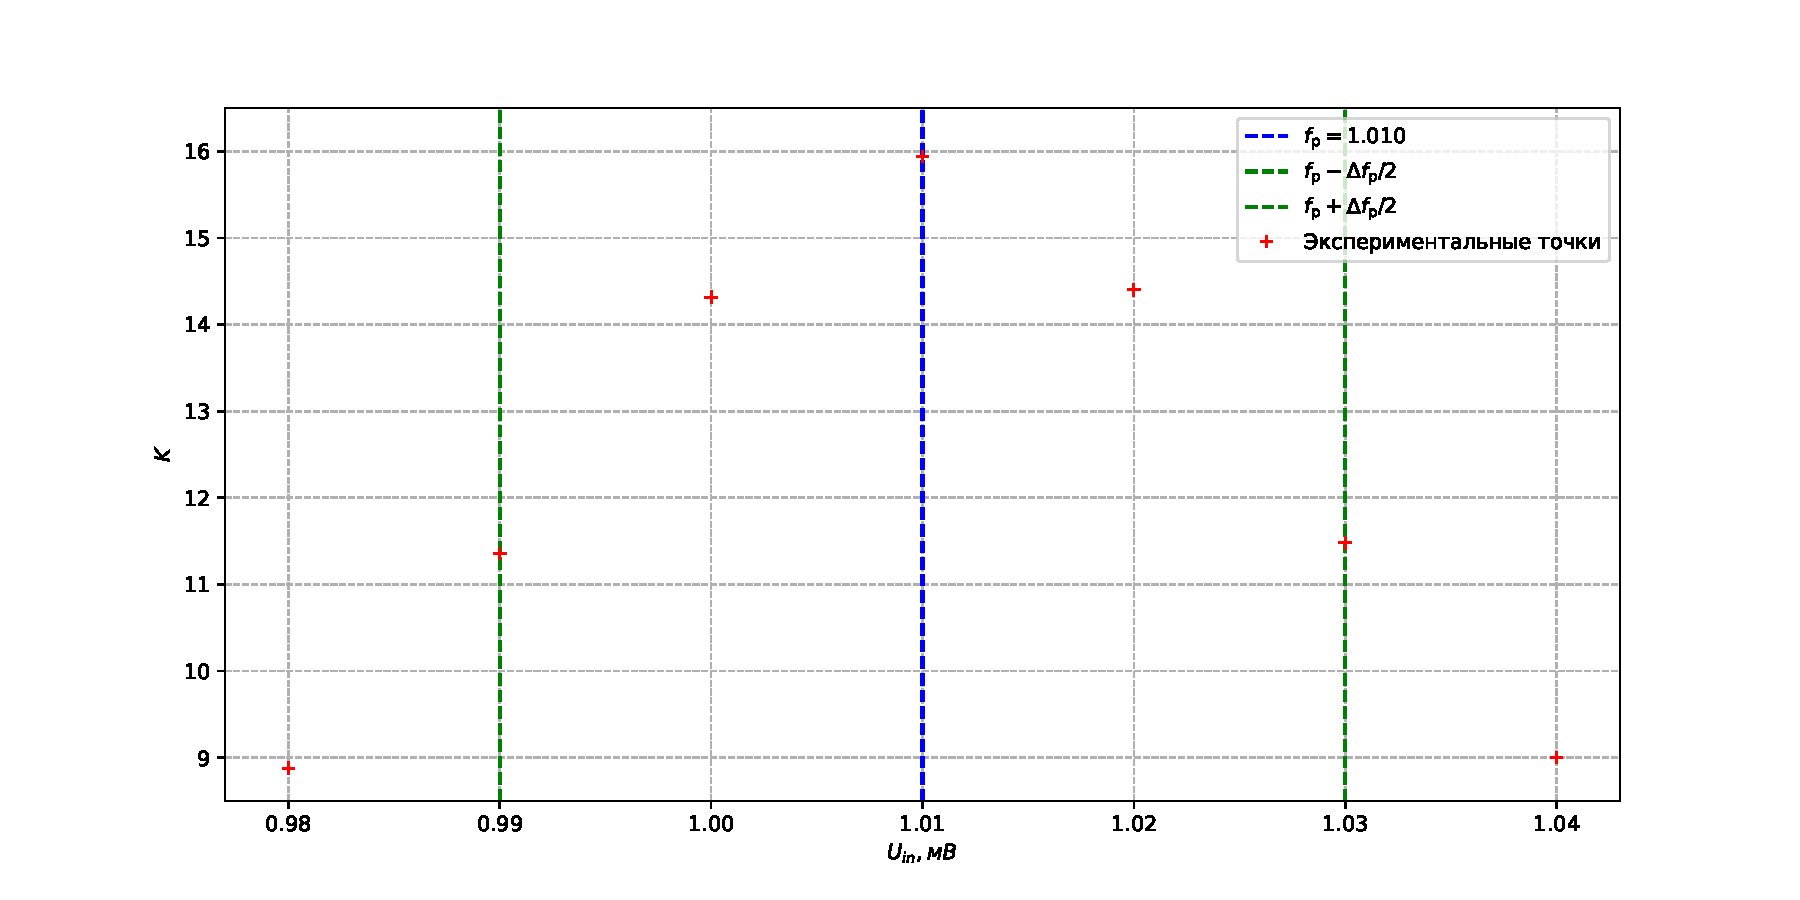
\includegraphics[width=\textwidth]{pictures/6_1_5_graph.pdf}
    \caption{Зависимость коэффициента усиления $K$ от частоты входного сигнала}
    \label{pic:graph-6-1-5}
\end{figure}

Максимальный коэффициент усиления равен $K_\text{max} = 15.94$. Уровень $K_\text{max}/\sqrt{2}$ достигается примерно на частотах $0.99~\text{МГц}$ и $1.03~\text{МГц}$, поэтому

\begin{equation*}
    \Delta f_\text{р} \approx 1.03 - 0.99 = 0.04~\text{МГц} = 40~\text{кГц}.
\end{equation*}

Добротность контура:

\begin{equation*}
    Q = \cfrac{f_\text{р}}{\Delta f_\text{р}} = \cfrac{1.01}{0.04} \approx 25.
\end{equation*}

\FloatBarrier

\subsection*{Кварцевый генератор с использованием последовательного резонанса кварца}

\begin{enumerate}
    \item Соберем схему кварцевого генератора с использованием последовательного резонанса кварца согласно рис. \ref{pic:ustan-6-2}.
\end{enumerate}

\begin{figure}[h]
    \centering
    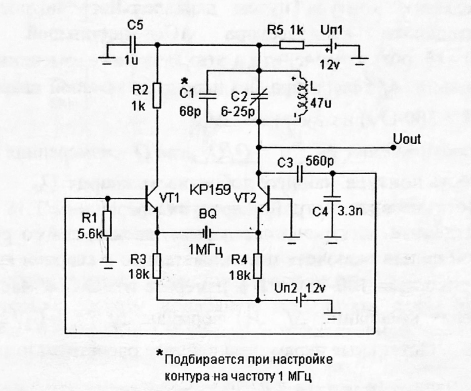
\includegraphics[width=0.75\textwidth]{pictures/ustan-6-2.png}
    \caption{Схема кварцевого генератора с использованием последовательного резонанса кварца}
    \label{pic:ustan-6-2}
\end{figure}

Сначала вместо кварцевого резонатора включим резистор $R = 300~\Omega$, примерно равный сопротивлению кварца на частоте последовательного резонанса. Частота и амплитуда колебаний:

\begin{equation*}
    f_0 = 1.014~\text{МГц},
    \qquad
    U_\text{out} = 9658~\text{мВ}.
\end{equation*}

\begin{enumerate}[resume]
    \item Восстановим схему кварцевого генератора, включив кварцевый резонатор вместо резистора. При $C_2 = 20~\text{пФ}$ амплитуда выходного сигнала равна
\end{enumerate}

\begin{equation*}
    A = 6000~\text{мВ}.
\end{equation*}

После изменения емкости и подстройки контура при $C_2 = 47~\text{пФ}$ получаем

\begin{equation*}
    A = 9130~\text{мВ}.
\end{equation*}

\begin{enumerate}[resume]
    \item Определим добротность кварцевого резонатора. Для этого расстроим контур дополнительной емкостью $\Delta C = 20~\text{пФ}$.
\end{enumerate}

Для генератора без кварца:

\begin{equation*}
    \Delta f = 994.0 - 974.0 = 20~\text{кГц}.
\end{equation*}

Для генератора с кварцем:

\begin{equation*}
    \Delta f_k = 1.001 - 0.995 = 6~\text{кГц}.
\end{equation*}

Из соотношения

\begin{equation*}
    \cfrac{\Delta f_k}{\Delta f} = \cfrac{Q}{Q_k}
\end{equation*}

найдем добротность кварца:

\begin{equation*}
    Q_k = Q \cfrac{\Delta f}{\Delta f_k} \approx 25 \cdot \cfrac{20}{6} \approx 83.
\end{equation*}

\begin{enumerate}[resume]
    \item Включим последовательно с кварцем конденсатор $C_s = 150~\text{пФ}$ и измерим изменение частоты:
\end{enumerate}

\begin{equation*}
    \Delta f_k = 1.001 - 0.998 = 3~\text{кГц}.
\end{equation*}

Из формулы

\begin{equation*}
    \cfrac{\Delta f_k}{f_k} = \cfrac{C_k}{2C_s}
\end{equation*}

получим

\begin{equation*}
    C_k = 2 C_s \cfrac{\Delta f_k}{f_k} \approx 1~\text{пФ}.
\end{equation*}

Остальные параметры кварцевого резонатора:

\begin{equation*}
    L_k = \cfrac{1}{4\pi^2 f_k^2 C_k} \approx 25~\text{мГн},
\end{equation*}

\begin{equation*}
    \rho_k = \cfrac{1}{2\pi f_k C_k} \approx 1.6 \cdot 10^5~\Omega,
\end{equation*}

\begin{equation*}
    r_k = \cfrac{\rho_k}{Q_k} \approx 1.9~\text{к}\Omega.
\end{equation*}

\begin{enumerate}[resume]
    \item Исследуем стабильность частоты при изменении питающего напряжения. Результаты измерений для схемы с резистором $R = 300~\Omega$ представлены в таблице \ref{tab:stability-6-2}.
\end{enumerate}

\begin{table}[!h]
    \centering
    \caption{Зависимость частоты генератора без кварца от питающего напряжения}
    \label{tab:stability-6-2}
    \begin{tabular}{|l|l|}
        \hline
        $U_\text{П}$, В & $f$, МГц \\ \hline
        -12 & 0.996 \\ \hline
        -11 & 0.997 \\ \hline
        -10 & 0.998 \\ \hline
        -9 & 0.994 \\ \hline
        -8 & 0.995 \\ \hline
        -7.2 & 0.996 \\ \hline
    \end{tabular}
\end{table}

Измеренная частота меняется слабо в пределах точности проведенных измерений:

\begin{equation*}
    f \approx \mathrm{const}.
\end{equation*}

\FloatBarrier

\subsection*{Кварцевый генератор с использованием кварца в качестве индуктивности}

\begin{enumerate}
    \item Соберем схему кварцевого генератора, в которой кварц используется как эквивалентная индуктивность, согласно рис. \ref{pic:ustan-6-3}.
\end{enumerate}

\begin{figure}[h]
    \centering
    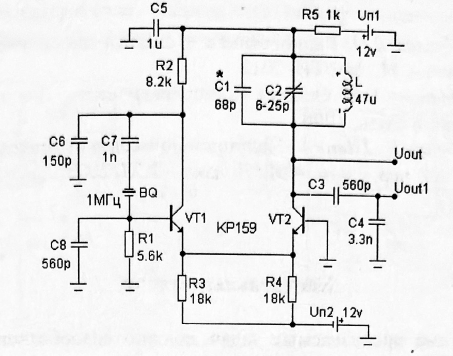
\includegraphics[width=0.75\textwidth]{pictures/ustan-6-3.png}
    \caption{Схема кварцевого генератора с использованием кварца в качестве индуктивности}
    \label{pic:ustan-6-3}
\end{figure}

Используемые емкости:

\begin{equation*}
    C_6 = 150~\text{пФ},
    \qquad
    C_7 = 1.02~\text{нФ},
    \qquad
    C_8 = 361~\text{пФ}.
\end{equation*}

Для последовательного соединения

\begin{equation*}
    C =
    \left(
        \cfrac{1}{C_6}
        +
        \cfrac{1}{C_7}
        +
        \cfrac{1}{C_8}
    \right)^{-1}.
\end{equation*}

По экспериментальным записям $C \approx 15~\text{пФ}$. Тогда расчетная частота генератора:

\begin{equation*}
    f_g =
    f_k
    \left(
        1 + \cfrac{C_k}{2C}
    \right)
    =
    1.034~\text{МГц}.
\end{equation*}

В пределах погрешности измеренная частота совпадает с расчетной.

\begin{enumerate}[resume]
    \item Изменим емкость $C_7$, подключив дополнительный конденсатор:
\end{enumerate}

\begin{equation*}
    C_7^{*} = 471~\text{пФ}.
\end{equation*}

Ожидаемое изменение частоты описывается формулой

\begin{equation*}
    \Delta f_g =
    -
    f_k
    \cfrac{\Delta C_3 C_k}{2 C_3^2}.
\end{equation*}

Знак минус означает, что при увеличении емкости частота уменьшается.

\begin{enumerate}[resume]
    \item Исследуем стабильность частоты генератора при изменении питающего напряжения. По результатам измерений существенного изменения частоты не наблюдалось:
\end{enumerate}

\begin{equation*}
    f \approx \mathrm{const}.
\end{equation*}

\section{Вывод}

В работе был исследован резонансный усилитель и два кварцевых генератора. Для резонансного усилителя была найдена резонансная частота $f_\text{р} = 1.01~\text{МГц}$, измерены амплитудная и частотная характеристики, а также оценена добротность контура $Q \approx 25$. При замыкании эмиттеров транзисторов коэффициент усиления заметно возрастает, что согласуется с уменьшением отрицательной обратной связи.

Для кварцевого генератора с использованием последовательного резонанса кварца была оценена добротность кварцевого резонатора $Q_k \approx 83$ и найдены его параметры: $C_k \approx 1~\text{пФ}$, $L_k \approx 25~\text{мГн}$, $\rho_k \approx 1.6 \cdot 10^5~\Omega$, $r_k \approx 1.9~\text{к}\Omega$. В схемах кварцевых генераторов частота оставалась практически постоянной при изменении питающего напряжения, что демонстрирует стабилизирующее действие кварцевого резонатора.

\end{document}
